\label{algorithms}
\subsection{Definitions}
Note that the graph $G = (V,E)$ describes a social network with $V$ denoting the set of nodes and $E$ the set of edges. Further, $|V| = n$, $|E| = m$ and $u,v$ are nodes of G. The set of neighbors of $u$ is denoted by $N(u)$ and the degree of node $u$ by $d_u=|N(u)|$. We will always assume $d_u\geq1\;\forall u$. Additionally, $f : V \rightarrow \{0,1\}$ is a binary function which takes a node $u \in V$ as input and outputs whether this node satisfies a certain property or not and $\bar{f} = \frac{1}{n}|\{u\;|\;f(u) = 1\}|$ is the fraction we wish to estimate.
The algorithms use $S$ as the set of nodes called \textit{sample} with $|S| = r$, the sample size.
We will denote the probability distribution by a a vector $p \in \mathbb{R}^n$ with $\sum_up_u = 1$.

Our goal is to achieve a good estimation of $\bar{f}$ using as little samples $S$ as possible with respect to an error bound $\epsilon$.
We introduce the concept of a set of algorithms called sampler which is defined as follows:
\begin{definition}[sampler]
  A sampler $\hat{f}(n,\epsilon,\delta)$ is a randomized algorithm with input $r$ (sample size), $\epsilon$ (sampler accuracy), $\delta$ (sampler error), $p$ (probability distribution) and function $f$ which outputs an expectation $\hat{f}$ with probability $1-\delta$ and $|\hat{f}-\bar{f}<\epsilon|$. Namely,
  $$\mathds{P}[|\hat{f}(n,\epsilon,\delta,p)-\bar{f} | > \epsilon] < \delta$$
  \label{defsampler}
\end{definition}

Note, that this definition of a sampler is in fact a special case of a statistical estimator.
Therefore we can analyze our sampler for estimator properties like bias and we sometimes denote our samplers as estimators.
\subsection{\texttt{Naive} sampler}
We will start by looking at an intuitive approach \cite{goldreich1997sample} for estimating $\bar{f}$ where we sample a set of nodes and poll each node $u$ to test if $f(u)=1$.
The algorithm will return the fraction of nodes that satisfy the condition and we call this approach the \texttt{Naive} sampler presented in pseudo code in Alg. \ref{algnaive}.

%---algo1----------------------------------------------
\begin{algorithm*}[!htb]
  \caption{\small {\bf Naive sampler}($G, f, r, p$)}
  \begin{code}
  {\bf Input:} Graph $G=(V,E)$, function $f : V \rightarrow \{0,1\}$, sample size $r$ \\
  {\bf Output:} $\hat{f}=\frac{1}{r}\sum\nolimits_{u\in S} f(u)$\\
  \\
  \uln \>\ubegin\\
  \uln \>\>initialize $f^*$ with 0 \\
  \uln \>\>randomly draw a set $S$ with r samples from $V$ with\\
  \>\>\>probability $p_u$ and with replacement\\
  \uln \>\>\ufor each $u \in S$ \udo\\
  \uln \>\>\>$f^* = f^* + f(u)$ \\
  \uln \>\>\uend\\
  \uln \>\ureturn $\hat{f} = f^*/r$ \\
  \uln \>\uend\\ 
  \end{code}
  \label{algnaive}
\end{algorithm*}
%---end algo2------------------------------------------
In the analysis we use a uniform distribution $p$ where we pick each node $u$ with probability $p_u = 1/n$.
\begin{theorem}
  The \texttt{Naive} sampler with sampling probability $p_u = 1/n$, accuracy $\epsilon$ and confidence $1-\delta$ requires $\frac{1}{2\epsilon^2}\ln{\frac{2}{\delta}}$ sample nodes
\end{theorem}
\begin{proof}
Recall that we want to poll $r$ uniformly chosen people independently and with replacement. The true fraction we want to approximate is $\bar{f}$. Let $F_u$ be the random variable for $f(u) = 1$.

It follows that $F_u \sim  Bernoulli(\bar{f})$ and $F_1, F_2, \ldots , F_r$ are independent.
Our \texttt{Naive} estimator is defined with $F = \sum_{u=1}^{r} F_u$ as $\hat{f} = F/r$.
We want our estimate to have accuracy $\epsilon$ and confidence $1-\delta$. This means that the probability that our estimation differs from the real value with a maximum of $\epsilon$ is larger than our defined confidence value (respectively $1-\delta$).
$$\mathds{P}[|\hat{f}-\bar{f} | \leq \epsilon] \quad\geq\quad 1-\delta$$
Since $F \sim Binomial(r,\bar{f})$, it follows
$$\textbf{E}[F] \quad=\quad \textbf{E}[\sum_{u=1}^{r} F_u] \quad=\quad \sum_{u=1}^{r}\textbf{E}[F_u] \quad=\quad r\bar{f}$$
We want to find a bound for the following expression:
$$\mathds{P}[|F-\textbf{E}[F] \geq r\epsilon] \quad=\quad \mathds{P}[|F-r\bar{f} \geq r\epsilon] \quad=\quad \mathds{P}[|\hat{f}-\bar{f} \geq \epsilon]$$ 
Using the two-sided Hoeffding's inequality the following holds for any $\epsilon \geq 0$
$$\quad \mathds{P}[|\hat{f}-\bar{f}|\geq \epsilon] \quad\leq\quad 2e^{-2r\epsilon^2}$$
%To achieve $\hat{f}$ bounded by $\epsilon$ we set $\epsilon = \gamma\bar{f}$, so $\gamma = \epsilon/\bar{f}$. Inserted in the formula above:
%$$\mathds{P}[|\hat{f}-\bar{f}| \geq \epsilon] \quad\leq\quad 2\exp (-\frac{\epsilon^2/\bar{f}^2}{2+\epsilon/\bar{f}}\cdot r\bar{f}) \quad=\quad 2\exp(-\frac{\epsilon^2}{2\bar{f}+\epsilon}\cdot r)$$
%Since the largest possible value of $\bar{f}$ is 1, if all nodes $u$ have $f(u) = 1$, the term in $\exp(\cdot)$ is an upper bound
%$$\frac{\epsilon^2}{2\bar{f}+\epsilon} \quad\geq\quad \frac{\epsilon^2}{2+\epsilon}$$
%and therefore
%$$\mathds{P}[|\hat{f}-\bar{f}| \geq \epsilon] \quad\leq\quad 2\exp(-\frac{\epsilon^2}{2+\epsilon}\cdot r)$$
Remember we want the confidence of the estimator bounded by $1-\delta$. We can also express this the other way around, which means the probability of an error larger than $\epsilon$ is less than $\delta$.
Therefore:
\begin{align*}
\quad&\mathds{P}[|\hat{f}-\bar{f} | > \epsilon] \quad\leq\quad \delta\\
&\Leftrightarrow\quad2e^{-2r\epsilon^2} \quad\leq\quad \delta\\
&\Leftrightarrow\quad e^{2r\epsilon^2} \quad\geq\quad \frac{2}{\delta}\\
&\Leftrightarrow\quad 2r\epsilon^2 \quad\geq\quad \ln\frac{2}{\delta}\\
&\Leftrightarrow\quad r \quad\geq\quad \frac{1}{2\epsilon^2}\ln{\frac{2}{\delta}} 
\end{align*}
%Since $\frac{2+\epsilon}{\epsilon^2}\ln\frac{2}{\delta}$ lies within $O(\frac{1}{\epsilon^2})$ this concludes the proof.$\hfill\square$
% We set the sample size $r = \frac{ln(2/\gamma)}{2\epsilon^2}$ and consider the set of nodes $S$ with elements $u$ being drawn independently and uniformly distributed.
% Using the Chernoff Bound the following inequality holds:
% $$P[$$ 
This matches the bound of $O(\frac{1}{\epsilon^2})$ proposed in the introduction and concludes the proof.
\end{proof}

Dasgupta et al. \cite{dasgupta2012social} proposed $r=2/(\epsilon^2\delta)$ and since $r=2/(\epsilon^2\delta) \geq \frac{1}{2\epsilon^2}\ln{\frac{2}{\delta}}$ this Lemma follows directly:
\begin{lemma}
Using $r=2/(\epsilon^2\delta)$ samples, with probability $1-\delta$ the \texttt{Naive} sampler will give an estimate $\hat{f}$ such that $|\hat{f}-\bar{f}|< \epsilon$.
\end{lemma}
\subsection{\texttt{Ideal} sampler}
We now want to improve our estimator by using the concept of social polling, so basically when we poll a node $u$ we expect to get an estimation of ${f(v)\;|\;v \in N(u)}$ to decrease the number of samples needed.
As briefly mentioned in the introduction the network structure is of great importance to the sampling method.
We will illustrate this on a small example. Consider a graph structure as shown in \rfig{network_a} where a single \texttt{RED} node is connected to several \texttt{BLUE} nodes.
Even though the portion of \texttt{RED} nodes is way smaller, using the \texttt{Naive} estimator the result is very biased towards the decision of {RED}.
%---figure network a------------------------------------
\begin{figure}[!ht]
  \begin{center}
    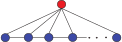
\includegraphics{fig1a}
    \caption{neighbor scaling}
    \lfig{network_a}
  \end{center}
\end{figure}
%---end figure network a--------------------------------

We introduce a social polling sampler called \texttt{Ideal} sampler that circumvents this bias by dividing each $f(v)$ by $d_v$. The pseudo-code is shown in Alg. \ref{algideal}.
We are going to provide a proof that this sampler is indeed unbiased and again present bounds on the sampling size.
%---algo2----------------------------------------------
\begin{algorithm*}[!htb]
\caption{\small {\bf Ideal sampler}($G, f, r, p$)}
\begin{code}
{\bf Input:} Graph $G=(V,E)$, function $f : V \rightarrow \{0,1\}$, sample size $r$,\\ distribution $p$ \\
{\bf Output:} $\hat{f}=\frac{1}{nr}\sum\nolimits_{u\in S}\frac{1}{p_u}\sum\nolimits_{v\in N(u)} f(v)/d_v$\\
\\
\uln \>\ubegin\\
\uln \>\>initialize $f^*$ with 0 \\
\uln \>\>randomly draw a set $S$ with r samples from $V$ with\\
\>   \>\>probability $p_u$ and with replacement\\
\uln \>\>\ufor each $u \in S$ \udo\\
\uln \>\>\>\ufor each $v \in N(u)$ \udo\\
\uln \>\>\>\>$f^* = f^* + \frac{1}{p_u}f(v)/d_v$ \\
\uln \>\>\>\uend\\
\uln \>\>\uend\\
\uln \>\ureturn $\hat{f} = \frac{f^*}{nr}$ \\
\uln \>\uend\\ 
\end{code}
\label{algideal}
\end{algorithm*}
%---end algo2------------------------------------------

First and foremost, we introduce $A$ as adjacency matrix of the graph $G$, which means $A_uv = 1$ if and only if $(u,v) \in E$. $D$ is called the diagonal matrix such that $D_{uu} = d_u$.
Let the diagonal matrix $P$ be $P_{uu} = p_u$ with $\sum\nolimits_{u}p_u$ for any vector $p \in \mathbb{R}^n$.
We also introduce $\mathds{F}$ which is the indicator (column) vector of the set ${u\;|\;f(u)=1}$, i.e., $\mathds{F}_u=f(u)$.
$\mathds{1}$ is simply an $n$-element vector of all 1's.
Our \texttt{Ideal} sampler is defined with $F = \sum_{u}\frac{e_u^TAD^{-1}\mathds{F}}{np_u}$ as $\hat{f} = F/r$.

\begin{lemma}
  The random variable $F$ satisfies $E[F] = \mathds{F}/n$ and \\
  $E[F^2] = \frac{1}{n^2}\mathds{F}^TD^{-1}AP^{-1}AD^{-1}\mathds{F}$.
\end{lemma}
\begin{proof}
\begin{align*}
\textbf{E}[F] \quad&=\quad \sum_u p_u \frac{e_u^TAD^{-1}\mathds{F}}{np_u} \quad=\quad \sum_u e_u^TAD^{-1}\mathds{F}/n \\
&=\quad\mathds{1}^TAD^{-1}\mathds{F}/n \quad=\quad DD^{-1}\mathds{F}/n \quad=\quad \mathds{F}/n \\
\textbf{E}[F^2] \quad&=\quad \sum_u p_u \bigg(\frac{e_u^TAD^{-1}\mathds{F}}{np_u}\bigg)^2 \quad=\quad \frac{1}{n^2}\sum_u \frac{(e_u^TAD^{-1}\mathds{F})^2}{p_u} \\
&=\quad\frac{1}{n^2}\sum_u \mathds{F}^TD^{-1}Ae_ue_u^TAD^{-1}\mathds{F}/p_u \\
&=\quad \mathds{F}^TD^{-1}A\bigg(\sum_ue_ue_u^T/p_u\bigg)AD^{-1}\mathds{F}/n^2 \\
&=\quad \mathds{F}^TD^{-1}AP^{-1}AD^{-1}\mathds{F}/n^2 \qedhere
\end{align*}
\end{proof}
Since $\mathds{F}/n$ is a vectorial way of expressing the fraction $\bar{f}$ the estimator is indeed unbiased.

We still want to find a bound for the number of samples, similar to the \texttt{Naive} sampler.
Therefore we first provide a bound for the variance in the special case where nodes $u$ are sampled with probability proportional $|N(u)| = d_u$.

\begin{lemma}
  Let the sampling probability be $p_u = \frac{d_u}{2m}$. Then $\textbf{var}(F) \leq (2m/n^2)\lambda_2^2||D^{-1/2}f||^2$ with $\lambda_2$ being the second largest eigenvalue of matrix $L = D^{-1/2}AD^{-1/2}$. 
\end{lemma}
\begin{proof}
\begin{align*}
\textbf{var}(F) \quad&=\quad \textbf{E}[F^2] - (\textbf{E}[F])^2 \quad=\quad \mathds{F}^TD^{-1}AP^{-1}AD^{-1}\mathds{F}/n^2 - (\mathds{F}/n)^2 \\
&=\quad \mathds{F}^TD^{-1}A(2mD^{-1})AD^{-1}\mathds{F}/n^2 - (\mathds{F}/n)^2\\
&=\quad \frac{2m}{n^2}\mathds{F}^TD^{-1}AD^{-1}AD^{-1}\mathds{F} - (\mathds{F}/n)^2\\
&=\quad \frac{2m}{n^2}\mathds{F}^TD^{-1/2}L^2D^{-1/2}\mathds{F}-\mathds{F}^T\mathds{1}\mathds{1}^T\mathds{F}/n^2\\
&=\quad \frac{2m}{n^2}\mathds{F}^TD^{-1/2}\bigg(L^2-\frac{D^{1/2}\mathds{1}\mathds{1}^TD^{1/2}}{2m}\bigg)D^{-1/2}\mathds{F}\\
&\leq\quad \frac{2m}{n^2}\bigg|\bigg|L^2 - \frac{D^{1/2}\mathds{1}\mathds{1}^TD^{1/2}}{2m}\bigg|\bigg|||D^{-1/2}\mathds{F}||^2
\end{align*}
In fact our recently defined matrix $L$ has interesting properties. For a graph $G$ we can compute the Laplacian matrix $\mathcal{L}$ as $\mathcal{L} = D - A$ where $A$ is the adjacency matrix and $D$ the degree matrix as defined above.
Taking $I-L$ is called the normalized Laplacian. Because of this association 
It can be shown that the second largest eigenvalue of $L^2 = \lambda_2^2 = ||L^2 - \frac{D^{1/2}\mathds{1}\mathds{1}^TD^{1/2}}{2m}||$ and therefore $1-\lambda_2$ is the second smallest eigenvalue of the normalized Laplacian. The proof then follows.
\end{proof}

We can now use this bound and the Chebyshev inequality to prove the following bound on $r$.
\begin{theorem}
Using $r = \frac{2\textbf{var}(F)}{\epsilon^2\delta}$ and $p_u = \frac{d_u}{2m}$, with probability $1-\delta$ the \texttt{Ideal} sampler will give an estimate $\hat{f}$ such that $|\hat{f}-\bar{f}|< \epsilon$.  
\end{theorem}
\begin{proof}
\begin{align*}
\mathds{P}[|\hat{f}-\bar{f}|\;>\epsilon] \quad&\leq\quad \frac{2\textbf{var}(\hat{f})}{\epsilon^2} \quad\leq\quad \frac{2\textbf{var}(\hat{F})}{r\epsilon^2} \\
&\leq\quad \frac{2\textbf{var}(F)\epsilon^2\delta}{2\textbf{var}(F)\epsilon^2} \quad\leq\quad \delta \qedhere
\end{align*}
\end{proof}
There are further, easier to compare bounds of the sample size if $G$ is $d-$regular and especially if the graph is an expander. Anyway, this requires a detailed look at the graphs properties and further investigations and is considered out of the scope of this paper \cite{alon1986eigenvalues}.
\subsection{\texttt{Sparse} sampler}
The \texttt{Ideal} sampler samples all neighbors of the sampled node. Thinking back to social network this means a person is expected to represent all of its neighbors choices.
Now, we present a variant of this estimator that only samples a subset $T_u$ of $u$'s neighbors.
This represents a scenario where either polling all neighbors is expensive respectively impossible (e.g. API limitations) or where we use further heuristics to select an arbitrary amount of neighbors. In the second case one could think of a poll like "\textit{Think of three of your female friends and tell us how many are married.}".

Be aware that this sampler uses an additional parameter called $k$. This is the size of set $T'_u$, a randomly chosen subset from $T_u$.
We are aware this contradicts the initial definition of a sampler but we since $k$ has no usage in the other samplers we will stick to this defintition.

In this implementation we will pick each neighbor with probability inversly proportional to their degrees and pick the subset of $k$ neighbors with probability $1/|T_u|$.
A pseudo code implementation is presented in Alg. \ref{algsparse}.

Providing a bound on variance and sample size is considered harder and not shown in this paper.
%---algo3----------------------------------------------
\begin{algorithm*}[!htb]
\caption{\small {\bf Sparse sampler}($G, f, r, p, k$)}
\begin{code}
{\bf Input:} Graph $G=(V,E)$, function $f : V \rightarrow \{0,1\}$, sample size $r$,\\ distribution $p$, parameter $k$ \\
{\bf Output:} $\hat{f}=\frac{1}{nr}\sum\nolimits_{u\in S}\frac{1}{p_u}(|T_u|/k)\sum\nolimits_{v\in T'_u} f(v)$\\
\\
\uln \>\ubegin\\
\uln \>\>initialize $f^*$ with 0 \\
\uln \>\>randomly draw a set $S$ with r samples from $V$ with\\
\>   \>\>probability $p_u$ and with replacement\\
\uln \>\>\ufor each $u \in S$ \udo\\
\uln \>\>\>1. randomly draw a set $T_u$ by picking each neighbor\\
\>   \>\>\> $v \in N(u)$ with probability $1/d_v$ \\
\uln \>\>\>2. randomly draw a set $T'_u \subseteq T_u$ by picking\\
\>   \>\>\> $k$ elements of $T_u$ without replacement with\\
\>   \>\>\> probability $1/|T_u|$.\\
\uln \>\>\>\ufor each $v \in T'_u$ \udo\\
\uln \>\>\>\>$f^* = f^* + \frac{1}{p_u}(|T_u|/k)f(v)$ \\
\uln \>\>\>\uend\\
\uln \>\>\uend\\
\uln \>\ureturn $\hat{f} = \frac{f^*}{nr}$ \\
\uln \>\uend\\ 
\end{code}
\label{algsparse}
\end{algorithm*}
%---end algo3------------------------------------------
\subsection{\texttt{Expectation} sampler}
The final presented sampler, short \texttt{Expec}, is based on the research and ideas of Rothschild and Wolfers in \cite{rothschild2009forecasting}. They showed with statistical measurements that using a method called \textit{expectation polling} can lead to significantly better estimations than the classical \textit{intent polling}.
In practise this means posing a "\textit{Which party will win the next vote?}" instead of "\textit{Who do you vote for?}".
They base this on the assumption that a respondent often gives an aggregate view of its friends and family (i.e. neighbors in a social network).
The presented algorithm Alg. \ref{algexpec} which aims to implement expectation polling lets each sampled node $u$ report a fraction instead of a simple 0 or 1. The fraction represents the estimated fraction of the neighbors with $f(v) = 1$.

Compared with the \texttt{Ideal} sampler there exist a similar bound on $r$ and we present this without a proof:
\begin{theorem}
Using $r = \frac{4m\lambda_2^2||D^{-1/2}\mathds{F}||||D^{-1/2}(\mathds{1}-\mathds{F})||}{n^2\epsilon^2\delta}$, with probability $1-\delta$ the \texttt{Expec} sampler will give an estimate $\hat{f}$ such that $|\hat{f}-\bar{f}|< \epsilon$.  
\end{theorem}
%---algo4----------------------------------------------
\begin{algorithm*}[!htb]
\caption{\small {\bf Expec sampler}($G, f, r, p$)}
\begin{code}
{\bf Input:} Graph $G=(V,E)$, function $f : V \rightarrow \{0,1\}$, sample size $r$,\\ distribution $p$ \\
{\bf Output:} $\hat{f}=\frac{1}{nr}\sum\nolimits_{u\in S}\frac{1}{p_u}G(u)$\\
\\
\uln \>\ubegin\\
\uln \>\>initialize $f^*$ with 0 \\
\uln \>\>randomly draw a set $S$ with r samples from $V$ with\\
\>   \>\>probability $p_u$ and with replacement\\
\uln \>\>\ufor each $u \in S$ \udo\\
\uln \>\>\>1. compute $q_u = \sum_{v\in N_u}\frac{f_v}{d_v}$\\
\>   \>\>\>2. compute $r_u = \sum_{v\in N_u}\frac{1}{d_v}$\\
\>   \>\>\>3. flip coin with probability $\frac{q_u}{r_u}$\\
\uln \>\>\>\uif heads\\
\uln \>\>\>\>$f^* = f^* + r_u$ \\
\uln \>\>\>\uelse\\
\uln \>\>\>\>$f^* = f^* + 0$ \\
\uln \>\>\>\uend\\
\uln \>\>\uend\\
\uln \>\ureturn $\hat{f} = \frac{f^*}{nr}$ \\
\uln \>\uend\\ 
\end{code}
\label{algexpec}
\end{algorithm*}
%---end algo4------------------------------------------
